\documentclass{standalone}

\usepackage{pgfplots}
\pgfplotsset{compat=newest}

\pagestyle{empty}

\newcommand{\aOne}{2.25}
\newcommand{\bOne}{0.8}
\newcommand{\scaleFactor}{0.065}

\begin{document}
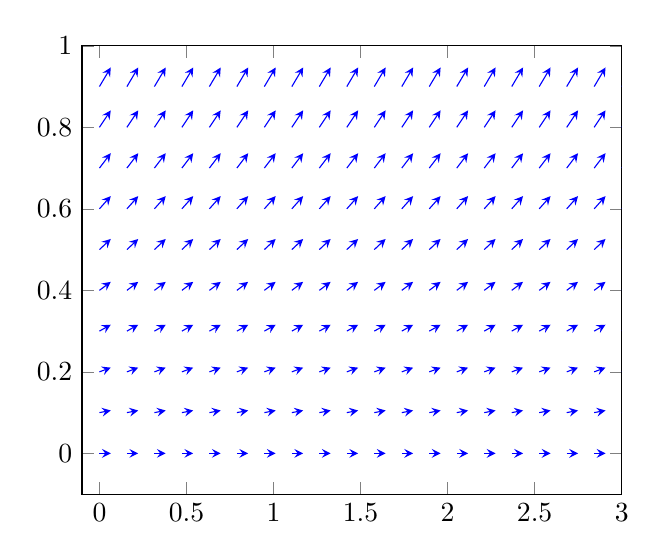
\begin{tikzpicture}
\begin{axis}[domain=0:3, xmin=-.1, xmax=3, ymin=-.1, ymax=1.]
	\addplot[red, domain=0:1] {\aOne*exp(\bOne*x)};
	\draw[red, very thick] 	plot file {y1.dat};
	\draw[blue, very thick] 	plot file {y2.dat};
	\draw[black, very thick] plot file {y3.dat};
	\addplot[blue, quiver={u=1,v=\bOne*y), scale arrows=\scaleFactor}, -stealth,samples=20] {0};
	\addplot[blue, quiver={u=1,v=\bOne*y), scale arrows=\scaleFactor}, -stealth,samples=20] {.1};
	\addplot[blue, quiver={u=1,v=\bOne*y), scale arrows=\scaleFactor}, -stealth,samples=20] {.2};
	\addplot[blue, quiver={u=1,v=\bOne*y), scale arrows=\scaleFactor}, -stealth,samples=20] {.3};
	\addplot[blue, quiver={u=1,v=\bOne*y), scale arrows=\scaleFactor}, -stealth,samples=20] {.4};
	\addplot[blue, quiver={u=1,v=\bOne*y), scale arrows=\scaleFactor}, -stealth,samples=20] {.5};
	\addplot[blue, quiver={u=1,v=\bOne*y), scale arrows=\scaleFactor}, -stealth,samples=20] {.6};
	\addplot[blue, quiver={u=1,v=\bOne*y), scale arrows=\scaleFactor}, -stealth,samples=20] {.7};
	\addplot[blue, quiver={u=1,v=\bOne*y), scale arrows=\scaleFactor}, -stealth,samples=20] {.8};
	\addplot[blue, quiver={u=1,v=\bOne*y), scale arrows=\scaleFactor}, -stealth,samples=20] {.9};
\end{axis}
\end{tikzpicture}
\end{document}
